\title{Quadratic Surfaces}
\subtitle{\SubTitleName}
\institute[]{\Course}
\author{\Instructor}
\maketitle   
  

\frame{\frametitle{Topics and Objectives}
    \Emph{Topics} \\
    %\TopicStatement
    \begin{itemize}
    
        % \item representing quadratic forms with symmetric matrices
        % \item Change of variables
        % \item Principle axes theorem
        \item classifying quadratic forms
    
    \end{itemize}
    
    \vspace{0.5cm}
    
    \Emph{Learning Objectives}\\
    
    %\LearningObjectiveStatement
    
    \begin{itemize}
    
        % \item characterize and classify quadratic forms using eigenvalues 
        % \item Express quadratic forms in the form $Q (\vec x ) =  \vec x ^{\, T} A \vec x$.
        % \item Apply the principle axes theorem to express quadratic forms with no cross-product terms.
        \item classify quadratic forms using the eigenvalues of the matrix of the quadratic form
        
    \end{itemize}
    
    \vspace{0.25cm} 
    


} 


\begin{frame}{Motivation}

    We will want to solve optimization problems of the form 
    $$\text{minimize } Q = ||A\vec x||^2 \text{, subject to constraints on } \vec x$$

    \begin{itemize}
        \item<2-> To help us understand this problem it is helpful to have a geometric interpretation of $Q = ||A\vec x||^2$.
        \item<3-> Recall that $Q = ||A\vec x||^2 = \vec x\,^T A^TA \vec x$ is a quadratic function, and $A^TA$ is symmetric.
        \item<4-> Terminology that describes the shape of $Q$ will also help us discuss the optimization problem.
    \end{itemize}
    
\end{frame}





\begin{frame}\frametitle{Curves in $\mathbb R^2$}

    \onslide<2->{Suppose $Q(\vec x) = \vec x^{\,T} A \vec x$, where $A \in \mathbb R^{2\times 2}$ is symmetric, and $C$ is a constant. } \onslide<3->{Then the set of $\vec x$ that satisfies $$C = \vec x^{\,T} A \vec x$$ defines a curve in $\mathbb R^2$.}
    
\end{frame}





\begin{frame}\frametitle{Example of a Curve in $\mathbb R^2$}

    $$Q = \vec x \, ^T \spalignmat{2 1;1 2} \vec x = 2x^2 +2y^2 +2xy=1$$ % the curves below represent various curves for $Q$ equal to 1, 2, 3.  
    
    \begin{center}
        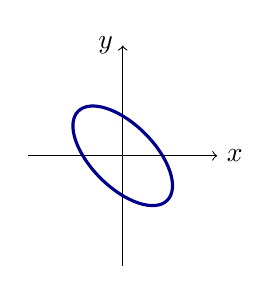
\begin{tikzpicture}[scale=0.4]
                \draw[->] (-3,0) -- (3,0) node[right] {$x$};
                \draw[->] (0,-3.5) -- (0,3.5) node[left] {$y$};
                \onslide<2->{\draw[rotate=45, DarkBlue, line width = 0.4mm] (0, 0) ellipse (1cm and 2cm);}
        \end{tikzpicture} 
        
    \onslide<3->{\textit{learning how to sketch such curves goes beyond the scope of this course}} % As we see on the next slide, the principle axes of the curve are related to the eigenvectors of $A$. 
    \end{center}  

\end{frame}





\begin{frame}\frametitle{Varying $C$}

    
    
    \begin{center}
    As we vary the value of $C$, the size of our ellipse will change. \\
    
    \vspace{12pt}
        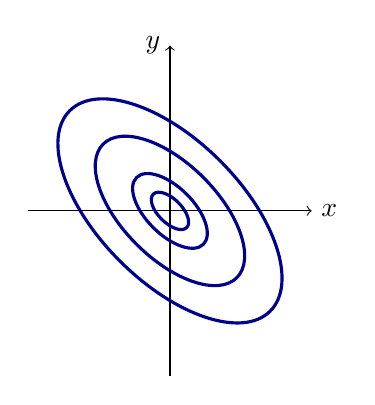
\begin{tikzpicture}[scale=0.6]
                \draw[->] (-3,0) -- (3,0) node[right] {$x$};
                \draw[->] (0,-3.5) -- (0,3.5) node[left] {$y$};
                \onslide<2->{\draw[rotate=45, DarkBlue, line width = 0.4mm] (0, 0) ellipse (1cm and 2cm);}
                \onslide<2->{\draw[rotate=45, DarkBlue, line width = 0.4mm] (0, 0) ellipse (1.5cm and 3cm);}
                \onslide<2->{\draw[rotate=45, DarkBlue, line width = 0.4mm] (0, 0) ellipse (.5cm and 1cm);}
                \onslide<2->{\draw[rotate=45, DarkBlue, line width = 0.4mm] (0, 0) ellipse (.25cm and .5cm);}
        \end{tikzpicture} 
        
    \onslide<3->{\textit{when we let $C$ vary continuously, we generate a surface in $\mathbb R^3$}} % As we see on the next slide, the principle axes of the curve are related to the eigenvectors of $A$. 
    \end{center}  

\end{frame}


\begin{frame}\frametitle{Surfaces}

    \onslide<1->{Suppose $z = Q(\vec x) = \vec x^{\,T} A \vec x$, where $A \in \mathbb R^{2\times 2}$ is symmetric. } \onslide<2->{Then the set of points that satisfy $$z = \vec x^{\,T} A \vec x$$ defines a surface in $\mathbb R^3$. }
    
\end{frame}







\begin{frame}\frametitle{Quadratic Forms as Surfaces}
    \vspace{-12pt}
    \begin{center}
    $$z = x^2 + y^2 = \vec x\, ^T \spalignmat{1 0;0 1}\vec x$$
    
    \tdplotsetmaincoords{70}{32}
    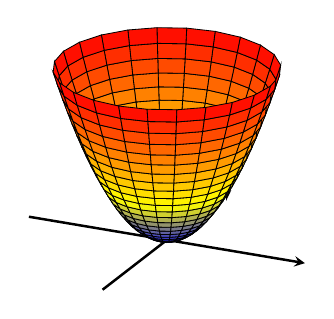
\begin{tikzpicture}[scale=.75]
        \begin{axis}[
            axis line style = very thick, smooth, no markers,
            xmin=-4,ymin=-4,zmin=0,xmax=4,ymax=4,zmax=10,
            axis lines=center,
            xticklabels={,,}, yticklabels={,,},zticklabels={,,},
            xtick=\empty, ytick=\empty, ztick=\empty, 
            % xlabel = $x$,ylabel=$y$,zlabel=$z$
            ]
        \addplot3 [surf,shader=flat,draw=black,draw=none,restrict z to domain=0:9, data cs=polar, domain=0:360, y domain=0:3] (x, y, y^2);
    \end{axis}    
    \end{tikzpicture}
    
    \vspace{12pt}
    
    \onslide<3->{\textit{notice that $z=0$ only at the origin}} 
    
    \end{center}
\end{frame}




\begin{frame} \frametitle{Surface Plots}
    
    $$Q = -4x^2 -2 y^2$$
    
    \vspace{12pt}
    \begin{center}
    
    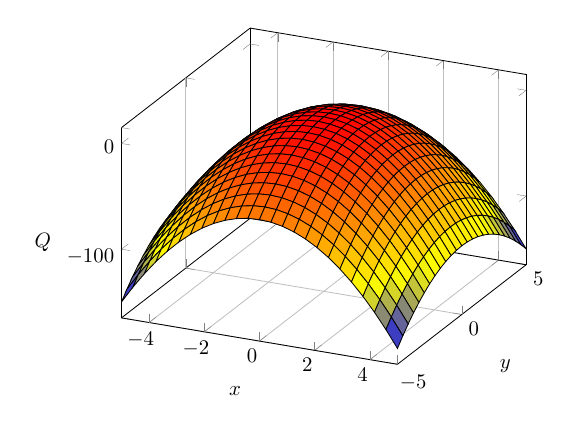
\begin{tikzpicture}[scale=0.75]
    \begin{axis} [xlabel = $x$,ylabel=$y$,zlabel=$Q$,ymajorgrids,xmajorgrids,zlabel style={rotate=270}] 
        \addplot3 [surf,shader=flat,draw=black] {-4*x^2 -2* y^2};
        \end{axis}
    \end{tikzpicture}
    \end{center}
    

\end{frame}

\begin{frame} \frametitle{Surface Plots}
    
    $$Q = 4x^2 + 2xy - 2y^2$$
    
    \vspace{12pt}

    \begin{center}
    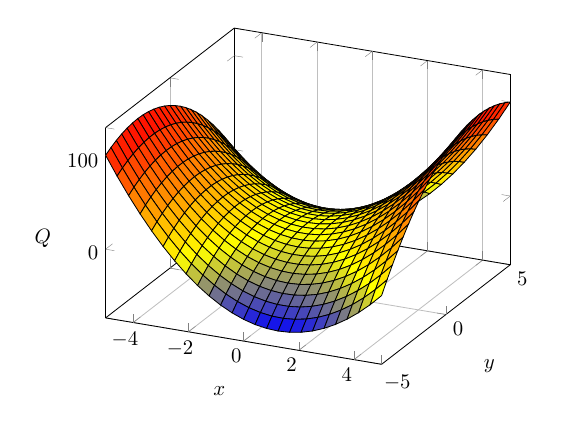
\begin{tikzpicture}[scale=0.75]
    \begin{axis} [xlabel = $x$,ylabel=$y$,zlabel=$Q$,ymajorgrids,xmajorgrids,zlabel style={rotate=270}] 
        \addplot3 [surf,shader=flat,draw=black] {4*x^2 + 2*x*y - 2*y^2};
        \end{axis}
    \end{tikzpicture}
    \end{center}
    

\end{frame}


% \begin{frame}\frametitle{Quadratic Forms as Surfaces}
%     \vspace{-12pt}
%     \begin{center}
%     $$z = -x^2 - y^2 = \vec x\, ^T \spalignmat{-1 0;0 -1}\vec x$$
    
%     \tdplotsetmaincoords{70}{32}
%     \begin{tikzpicture}[scale=.75]
%         \begin{axis}[
%             axis line style = very thick, smooth, no markers,
%             xmin=-4,ymin=-4,zmin=0,xmax=4,ymax=4,zmax=10,
%             axis lines=center,
%             xticklabels={,,}, yticklabels={,,},zticklabels={,,},
%             xtick=\empty, ytick=\empty, ztick=\empty, 
%             % xlabel = $x$,ylabel=$y$,zlabel=$z$
%             ]
%         \addplot3 [surf,shader=flat,draw=black,draw=none,restrict z to domain=-9:0, domain=0:360, y domain=0:3] (x, y, -x^2 -y^2);
%     \end{axis}    
%     \end{tikzpicture}
    
%     \vspace{12pt}
    
%     \onslide<3->{\textit{notice that $z=0$ only at the origin}} 
    
%     \end{center}
% \end{frame}





\begin{frame}\frametitle{Classifying Quadratic Forms}
    
    \begin{center}\begin{tikzpicture} \node [mybox](box){\begin{minipage}{0.90\textwidth}\vspace{2pt}
        A quadratic form $Q$ is 
        \begin{itemize}
            \item<2-> \Emph{positive definite} if $Q > 0$ for all $\vec x \ne \vec 0$.
            \item<2-> \Emph{negative definite} if $Q<0$ for all $\vec x \ne \vec 0$.
            \item<3-> \Emph{positive semidefinite} if $Q\ge0$ for all $\vec x$.
            \item<3-> \Emph{negative semidefinite} if $Q\le0$ for all $\vec x$.
            \item<4-> \Emph{indefinite} if $Q$ takes on positive and negative values for $\vec x \ne \vec 0$.
        \end{itemize}
    \end{minipage}};
    \node[fancytitle, right=10pt] at (box.north west) {Definition};
    \end{tikzpicture}\end{center}    

\end{frame}



\begin{frame}\frametitle{Quadratic Forms and Eigenvalues}

    \begin{center}\begin{tikzpicture} \node [mybox](box){\begin{minipage}{0.90\textwidth}\vspace{2pt}
    
        \linespread{1.5}
    
        If $A$ is a symmetric matrix with eigenvalues $\lambda_i$, then $Q = \vec x^{\,T} A \vec x$ is 
        
        \begin{itemize}
            \item \onslide<2->{\Emph{positive definite} when all eigenvalues are positive}
            \item \onslide<2->{\Emph{negative definite} when all eigenvalues are negative}
            \item \onslide<3->{\Emph{indefinite} when at least one eigenvalue is negative and at least one eigenvalue is positive}
        \end{itemize}
        
    \end{minipage}};
    \node[fancytitle, right=10pt] at (box.north west) {Theorem};
    \end{tikzpicture}\end{center}
\end{frame}



\begin{frame}\frametitle{Quadratic Forms and Eigenvalues}    
    \Emph{Proof}: assuming $A$ symmetric, we can write $A=PDP^T$ and set $\vec x = P\vec y$, so
    \begin{align*}
        \onslide<2->{Q = \vec x \,^T A\vec x 
                    &= (P\vec y)^T A (P\vec y) \\}
        \onslide<3->{ &= \vec y\, ^T P^T A P\vec y \\}
        \onslide<4->{ &= \vec y\, ^T D\vec y , \quad \text{using } A = PDP^T \\}
        \onslide<5->{&= \sum \lambda_i y_i^2, \quad \text{because } D \text{ is diagonal}}
    \end{align*}
    \onslide<6->{
    Because $y_i^2$ is always non-negative, for $\vec y \ne 0$, 
    \begin{itemize}
        \item $Q$ is positive when, for all $i$, $\lambda_i >0 \quad \Rightarrow \quad Q $ is positive definite
        \item $Q$ is negative when, for all $i$, $\lambda_i < 0 \quad \Rightarrow \quad  Q$ is negative definite
        \item indefinite when $\lambda_i$ has both negative and positive values
    \end{itemize}
    }
    
    
\end{frame}



\begin{frame}\frametitle{Quadratic Forms and Eigenvalues Example}        

    $$\onslide<1->{Q = 4x^2 + 2xy - 2y^2 = \vec x\,^T A \vec x} \onslide<2->{\Rightarrow A = \spalignmat{4 1;1 -2}, \quad \lambda = 1 \pm \sqrt{10} }$$
    
    \vspace{-6pt}
    
    \onslide<3->{
    \begin{center}
    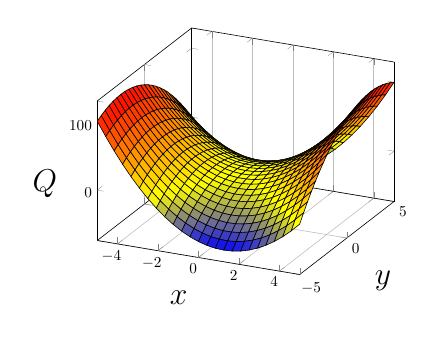
\begin{tikzpicture}[scale=0.55]
    \begin{axis} [xlabel = $x$,ylabel=$y$,zlabel=$Q$,ymajorgrids,xmajorgrids,zlabel style={rotate=270},xlabel style={font=\huge},ylabel style={font=\huge},zlabel style={font=\huge}] 
        \addplot3 [surf,shader=flat,draw=black] {4*x^2 + 2*x*y - 2*y^2};
        \end{axis}
    \end{tikzpicture}
    
    \textit{eigenvalues are both positive and negative $\Rightarrow$ $Q$ is indefinite}
    
    \end{center}
    }


\end{frame}

\frame{\frametitle{Summary}

    \SummaryLine \vspace{4pt}
    \begin{itemize}\setlength{\itemsep}{8pt}

        \item the classification of quadratic forms using eigenvalues

    \end{itemize}
    
    \vspace{6pt}

    
}